%!TEX root = ../main.tex
%%%%%%%%%%%%%%%%%%%%%%%%%%%%%%%%%%
% Links:
%
% Difficulty: Companies: 
%%%%%%%%%%%%%%%%%%%%%%%%%%%%%%%%%%


%\begin{figure} \centering 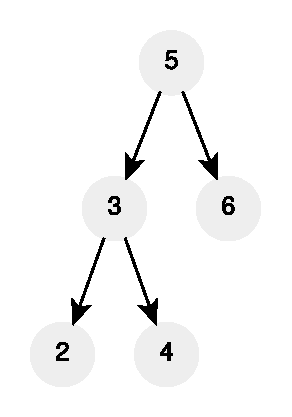
\includegraphics[width=\textwidth]{sources/decode_string/images/example1}
%   \caption[Sample short cpation]{Sample Caption}. \label{fig:decode_string:example1} \end{figure}

\chapter{Decode the message}
\label{ch:decode_string}
\section*{Introduction}
The problem in this chapter resembles the one for decoding a string encoded with the famous \textit{run-length
encoding method}(RLE).
RLE is a simple form of data compression in which a stream of data is
given (e.g. \quotes{AAABBCCCC}) and the output is a sequence of counts of consecutive
data values in a row. (e.g. \quotes{3A2B4C}).
It is a type of lossless encoding meaning that the encoding
process does not lose any information in the original input and therefore the input data can be recovered fully and integrally decoded. 

This chapter will deal with a similar algorithm where we will be asked to write a function capable of decoding a string encoded with a run-length-encoding-like algorithm. More than complicated insights, string manipulation skills and attention to details of the implementation and for corner cases are going to be crucial in order to solve this problem during an actual interview. 

\section{Problem statement}
\begin{exercise}
\label{example:decode_string:exercice1}
Write a function that given an encoded string $s$  decodes it. $s$ is of the form:
${k_1[d_1]k_2[d_2[ \ldots]}$ where $k$ is a positive integer and $s$ is another encoded string. The
decoded version of $s$ is obtained by appending $d_1$ $k_1$ followed by repeating $d_2$ $k_2$ times.
 
	%example1
	\begin{example}
		\label{example:decode_string:example1}
		\hfill \\
		Given \inline{s="2[abc]3[ab]"} the function returns \inline{"abcababababcababab"}.
	\end{example}

	%example2
	\begin{example}
		\label{example:decode_string:example2}
		\hfill \\
		Given \inline{s="2[abc3[ab]]"} the function returns \inline{"abcababababcababab"}.
	\end{example}

	\begin{example}
		\hfill \\
		Given \inline{s="2[abc]3[cd]ef"} the function returns \inline{"abcabccdcdcdef"}.

	\label{ex:decode_string:example3}
	\end{example}
\end{exercise}

\section{Clarification Questions}

\begin{QandA}
	\item \begin{questionitem} \begin{question} Is it guaranteed that $s$ is always valid?  \end{question} 	 
    \begin{answered}
		\textit{Yes, $s$ contains only lower-case letters from the English alphabet, numbers and square brackets and it is a valid encoded string.}
	\end{answered} \end{questionitem}

	\item \begin{questionitem} \begin{question} Is there an upper-bound on the size of the encoded-substrings (the $k$s in the problem statement)?  \end{question} 	 
		\begin{answered}
			\textit{Not really, you are only guaranteed their value to fit into a built-in \inline{int}.}
		\end{answered} \end{questionitem}

\end{QandA}

\section*{Discussion}
\label{decode_string:sec:discussion}


\subsection{Recursive solution}
\label{decode_string:sec:recursive}
The first thing to note about this problem is that the encoded string has a recursive definition.
Whenever we encounter a number $k$ followed by the closed square bracket character  \inline{'['} 
we know that we have
to decode whatever is inside the brackets and replicate it $k$ times.
We can use this fact to simply create a recursive algorithm which follows this definition.
The real challenge of this problem actually lies in the implementation more than in the algorithm itself and in our opinion specifically in the correct parsing of the string.

The idea is to construct the final answer by looking at one character of $s$ at a time. We can start
from  the char at index $0$ and depending on what it is:
\begin{enumerate}
	\item append it to the answer (when $s$ an alphabetic letter);
	\item parse it as a part of a number (when $s$ is a digit);
	\item recursively decode the rest of the string (when $s$ is an open square bracket \inline{'['}).
\end{enumerate}

For instance, let's assume we have to decode \inline{s="xy242[ab3[c]de]}.
We start by reading \texttt{'x'} and \texttt{'y'} which are letters and therefore are
just appended to the final answer.
We then see a digit which tells us that a number has started. 
We parse all of its digits into the integer $242$ (which assumes we need to perform a conversion from string to int; see Chapter \ref{ch:string_to_int} at page \pageref{ch:string_to_int} where we delved into it for a refresher).
The end of the number is signaled by the presence of the char
\inline{'['} which also signals that a new encoded substring is starting.
So when we see an open
square bracket character we recursively call the decode function so that it returns the expansion of
whatever is within the brackets.
When the recursive call ends (when we find a closed square bracket
character \inline{']'}) we are left with the expanded string which we can then replicate $242$ times
and append to the final answer.
When a recursive call ends the caller must continue processing the elements of $s$ from the last unprocessed character.
We keep track of the next element to be processed via a integer variable which is passed along to each of the recursive calls.
This is necessary because after the
recursive call returns we might need to continue processing more characters. Regarding the example above, when the recursive call 
associated with the substring \inline{3[c]} returns we still have to process \inline{de} for the encoded substring substring 
\inline{ab3[c]de}.

Listing \ref{list:decode_string:recursive} shows a possible implementation of this idea. 


\lstinputlisting[language=c++, caption={Recursive implementation of the algorithm described in Section \ref{decode_string:sec:recursive}},label=list:decode_string:recursive]{sources/decode_string/decode_string_solution2.cpp}

Notice that the function \inline{decode_string_recursive_helper} takes the second parameter 
as a reference to an integer.
As mentioned above already, we use a reference because we want this number 
to be updated by each of the recursive calls and this way we do not lose track of what portion of the input is still to be processed.
The variable $i$ to keep track of the current character we are examining in $s$. 
Figure \ref{fig:decode_string:recursion} graphically depicts and describes the execution 
of this algorithm  on the input string \inline{ab23[x12[w]]cd}.

The time and complexities of the code in Listing \ref{list:decode_string:recursive} is $O(K|s|)$ where $k$ is the largest replication factor we can have.

\begin{figure}
	
	\vspace{-3.5cm}

	\captionsetup{font=footnotesize,labelfont=footnotesize}
	\centering
	\hspace*{-1.5cm}
	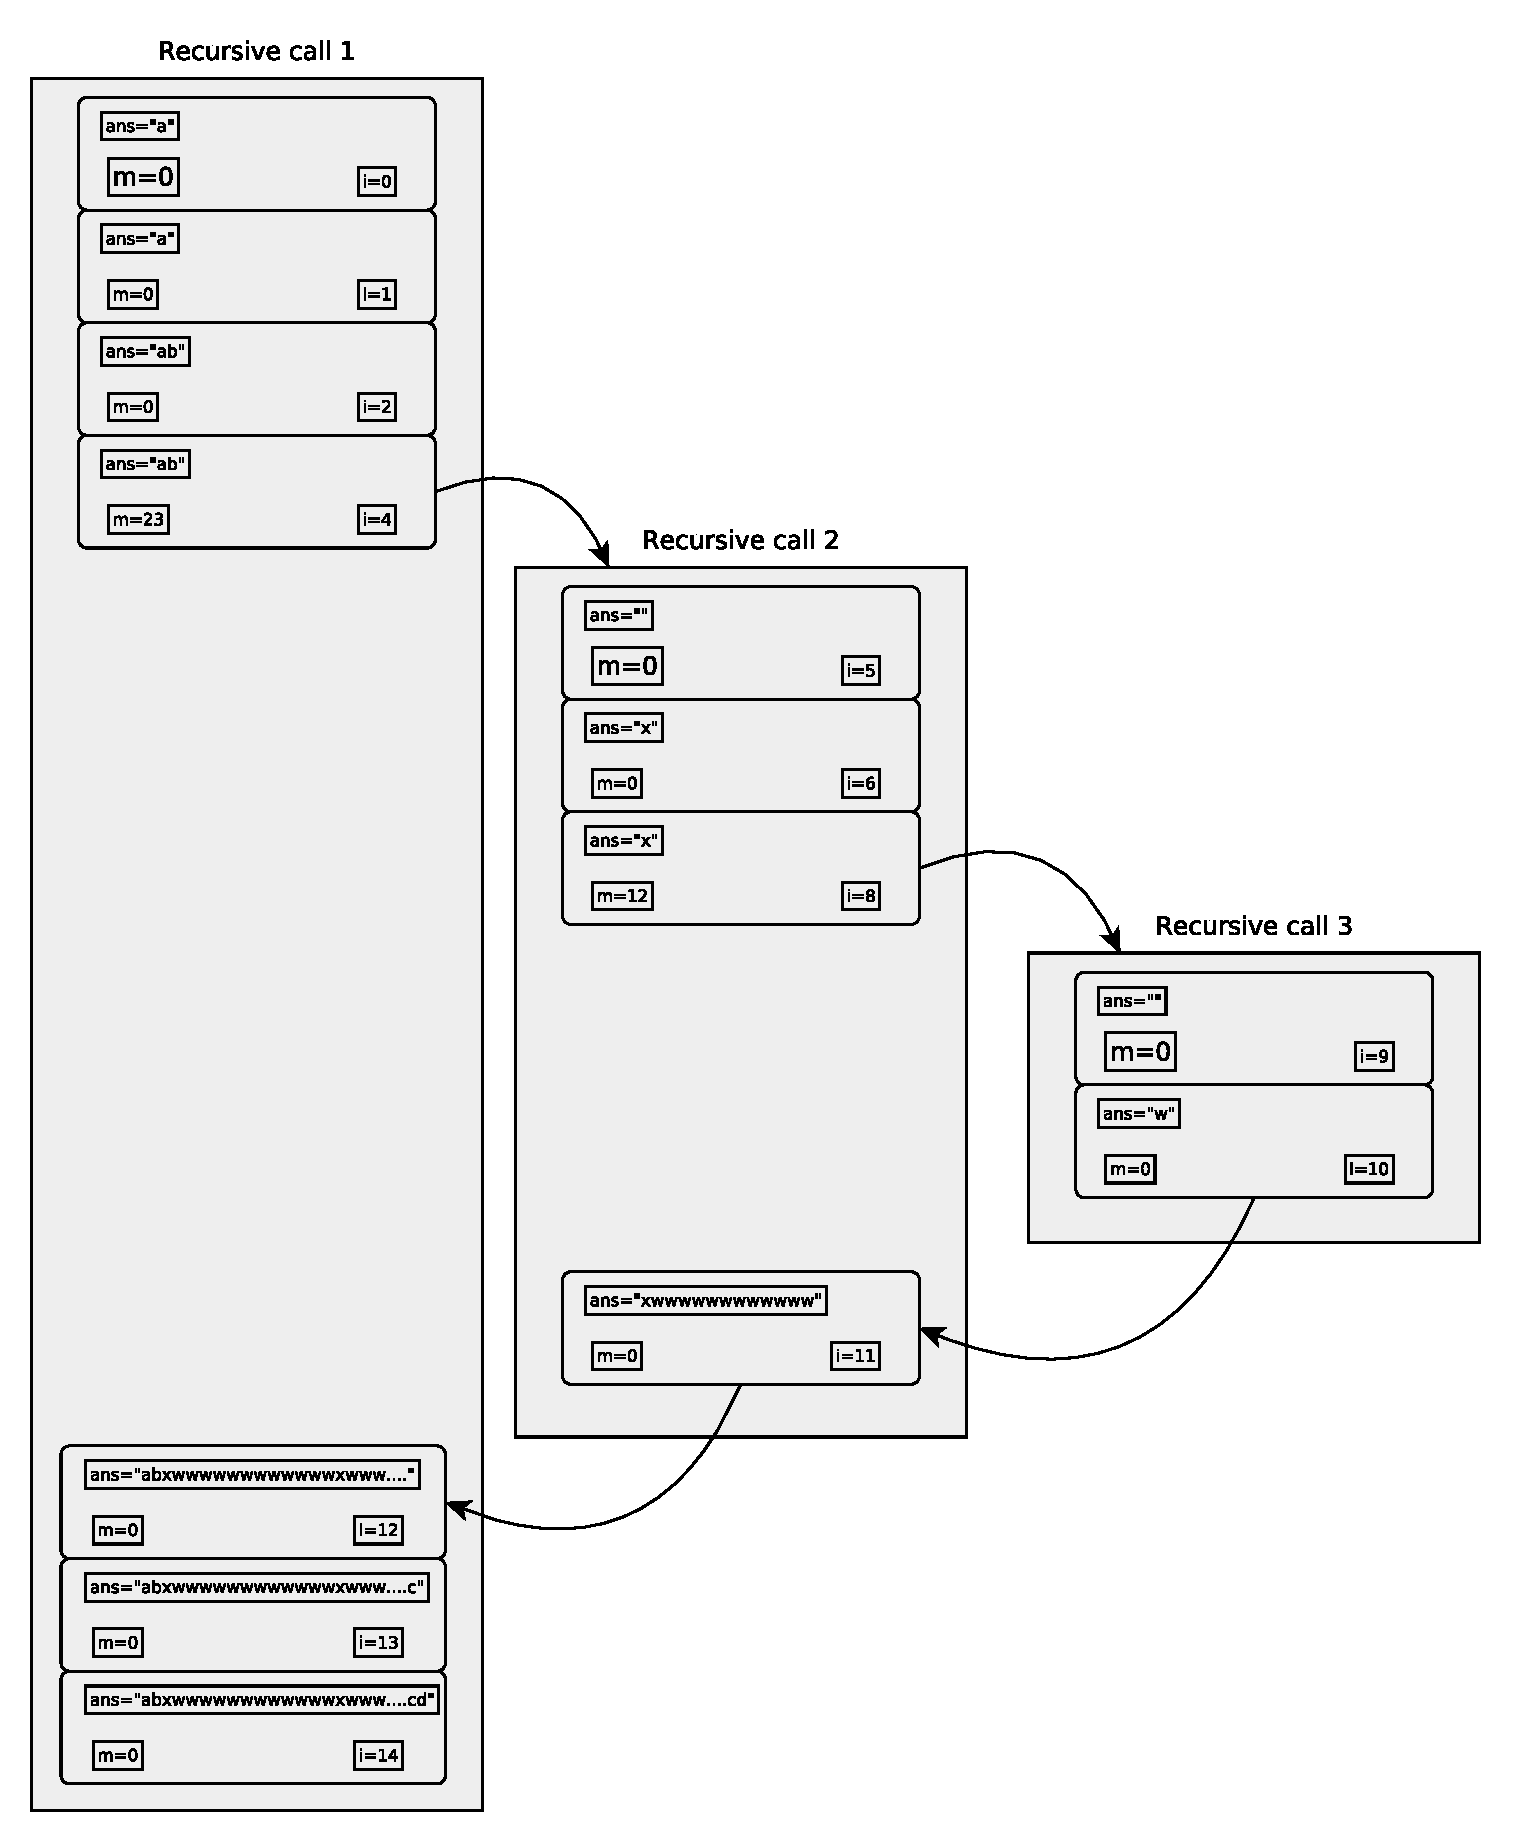
\includegraphics[width=1.25\textwidth]{sources/decode_string/images/recursion}
	\vspace*{-10mm}
   \caption{Execution of the algorithm in Listing \ref{list:decode_string:recursive} for the input
	string \inline{s="ab23[x12[w]]cd}. The execution starts (Figure (a)) with a first call to
	\inline{decode_string_recursive_helper} with \inline{i=0}. The first two characters are letters
	and therefore they are appended to the instance of \inline{ans} bounded to this recursive call
	(Figures (a) and (b)). Characters at indices $2$ and $3$ are numbers and they are parsed and
	saved into the integer \inline{m} (Figure (c)). The next character is going to be the open
	square bracket at index $4$  and this will cause a new recursive call to happen with $i=5$
	(Figure (d)). The process repeats now and we see at index $5$ a letter that we append to the
	instance of \inline{ans} bound to this call (Figures (e)). We then parse the number $12$ at
	characters $6$ and $7$ (Figure (f)) and subsequently at index $8$ we find an open square bracket
	that leads to a new recursive call, this time starting from index $i=9$ (Figure (g)). Index $9$ holds
	a letter which is appended to the (empty) instance of \inline{ans} bound to this call (Figure
	(h)). The next character is a closed square bracket which mean we can terminate the recursive
	call and return to the caller \inline{ans} (which now holds \inline{"w"}). We are not back
	(Figure (k)) to the second recursive call where, as you remember, $m$ is twelve. Therefore we
	replicate $12$ times the string we received from the recursive call number three and append the
	result to the current instance of \inline{ans}. We also set $m$ to zero. Because the next
	character is again a closed bracket we return the the caller and repeat the process (Figure
	(i)).$m=23$ and therefore we replicate \inline{ans} from the second recursive call $23$ times.
	The rest of the characters left are the ones at indices $11$ and $12$ which are simple letters
	and are just appended to \inline{ans}.}	
   \label{fig:decode_string:recursion}
 \end{figure}

 \subsection{Iterative solution}
 \label{decode_string:sec:iterative}
The same idea can of course be implemented iteratively. The trick is to \textit{simulate} the call
stack of the recursive approach in Section \ref{decode_string:sec:recursive} by using an explicit
stack. This stack will contains two pieces of information 
\begin{enumerate*}
	\item the replication factor associated with an encoded substring (the value $1$ is the default)
	\item the decoded substring
\end{enumerate*}. 
	
Initially the stack contains only one entry: \inline{(1,"")}. 
As in the recursive approach, we process $s$ one character at a time and all the
operations are performed on the \textbf{top} of the stack unless we encounter either a: 
\begin{itemize}
	\item \inline{'['} which
	signals we need to add another element to the stack and start decoding a substring of $s$.
	\item \inline{']'} which signals that we are done with decoding the substring and we can then replicate it
	as many time as is necessary, remove the entry from the top of the stack and append the replicated
	string to the string associated with the new top of the stack.
\end{itemize}
At the end of this process we are
left with the fully decoded string at the top of the stack.

Listing \ref{list:decode_string:iterative} implements this idea.

\lstinputlisting[language=c++, caption={Iterative solution using a \inline{std::stack}.},label=list:decode_string:iterative]{sources/decode_string/decode_string_solution1.cpp}
 
Notice that the stack has type
\inline{std::stack<std::pair<int,std::string>>} thus reflecting the fact we need to keep two pieces of 
information for each of the encoded substrings.
As for the recursive implementation, both time and space complexities are $O(K|s|)$.